\documentclass[conference]{IEEEtran}

\usepackage{cite}
\usepackage{amsmath,amssymb,amsfonts}
\usepackage{graphicx}
\usepackage{textcomp}
\usepackage{xcolor}
\usepackage{url}

\graphicspath{{figures/}}

\begin{document}

\title{Cost-Aware Conditional Diffusion Compression of 4K-5K Drone Imagery for Scalable High-Performance Computing Workflows}

\author{
\IEEEauthorblockN{Jooho Kim\IEEEauthorrefmark{1}, Anish Shakya\IEEEauthorrefmark{2}, Yifan Yang\IEEEauthorrefmark{2}, and Jacob Kelly\IEEEauthorrefmark{2}}
\IEEEauthorblockA{\IEEEauthorrefmark{1}Institute for a Disaster Resilient Texas, Texas A\&M University, College Station, TX, USA}
\IEEEauthorblockA{\IEEEauthorrefmark{2}Texas A\&M University, College Station, TX, USA}
\IEEEauthorblockA{Corresponding author: \texttt{jooho.kim@tamu.edu}}
}

\maketitle

\begin{abstract}
High-resolution drone imagery supports detailed disaster assessment, object mapping, and recovery planning, but 4K-5K imagery creates a difficult data-management problem for high-performance computing (HPC) workflows. Full-resolution image archives increase storage cost, data movement, GPU memory pressure, and turnaround time for downstream analysis. This paper studies conditional diffusion compression (CDC) as a cost-aware strategy for managing large drone-image collections on GPU HPC systems. We adapt a CDC reconstruction and compression workflow to NCSA DeltaAI, run controlled experiments on full-resolution drone images cropped to $5440 \times 3648$ pixels, and measure runtime, GPU memory, compression ratio, PSNR, SSIM, pixel-error statistics, and tiling artifacts. The experiments show that native full-image processing is feasible but memory-heavy, using about 52 GB of GPU memory and 144 seconds per image in the baseline configuration. A selected $256 \times 256$ tiling configuration reduces runtime by 44.7\% and peak GPU memory by about 31.3$\times$ relative to no tiling while keeping PSNR and SSIM close to the full-image reference. Resolution reduction gives large speedups but noticeably degrades quality, and larger batch sizes do not improve throughput in the controlled 2K setting. The results identify tiling and checkpoint selection as the most practical near-term controls for scalable CDC-based drone imagery workflows.
\end{abstract}

\begin{IEEEkeywords}
conditional diffusion compression, drone imagery, high-performance computing, lossy compression, GPU memory, tiling
\end{IEEEkeywords}

\section{Introduction}

Drone imagery is increasingly used after floods, storms, and other disasters because it provides local visual evidence at a spatial detail that satellite imagery often cannot supply. The same resolution that makes these images useful also makes them costly to store and process. A single full-resolution frame in the current workflow has $5440 \times 3648$ pixels; as uncompressed RGB, that image contains about 59.5 MB of pixel data. A field campaign with thousands of such frames can quickly become a storage, transfer, and GPU scheduling problem before the research team reaches the downstream mapping or assessment task.

Lossy neural compression offers a way to reduce that burden, but disaster-imagery workflows need more than a low bitrate. They need predictable reconstruction time, bounded GPU memory, reproducible quality checks, and output artifacts that can be inspected by humans. Conditional diffusion compression is attractive because it can reconstruct visually plausible image content from a compact latent representation \cite{yang2022lossy}. At the same time, diffusion decoding is iterative. If the denoising process is too slow or too memory-intensive, the compression scheme becomes difficult to use in HPC production workflows.

This paper studies the system-level operating conditions for CDC-based drone-image compression on GPU HPC hardware. The goal is not to introduce a new compression architecture. Instead, we ask a practical question: under what settings can an existing CDC workflow become fast, memory-efficient, and inspectable enough for large disaster-imagery workloads?

The paper makes three contributions. First, it adapts a CDC compression and reconstruction workflow to NCSA DeltaAI and defines a repeatable experiment suite for native images, downsampled images, batch-size sweeps, checkpoint sweeps, storage placement, and tiled reconstruction. Second, it reports measured trade-offs for full-resolution drone imagery on GH200-class hardware, including runtime, memory, compression ratio, PSNR, SSIM, and pixel-error statistics. Third, it identifies a selected $256 \times 256$ tiling configuration that sharply reduces memory and runtime while preserving comparable image-quality metrics and avoiding obvious tile-boundary artifacts in the inspected visual examples.

% TODO: Add a full related-work section after the core experimental narrative stabilizes.

\section{Problem Setting and Design Goals}

\subsection{Workflow Setting}

The target workflow starts from high-resolution drone images, compresses them with a pretrained CDC model, reconstructs them for analysis, and stores lightweight quality evidence for review. The repository separates two operational questions. The compression-side question asks how quickly the data can be reduced and which bitrate-quality settings are practical. The reconstruction-side question asks how quickly the compressed data can be used again, especially when full-resolution decoding stresses GPU memory.

The workflow uses the x-parameterized CDC path from the original model implementation \cite{yang2022lossy}. In this path, the compression setting is controlled by the checkpoint rather than by a runtime quality argument. The experiment suite therefore treats checkpoint selection as the main compression-level control and uses measured bits per pixel (BPP) and compression ratio to label low-, balanced-, and high-compression operating points.

\subsection{Design Goals}

The workflow is designed around four practical goals.

\begin{itemize}
\item \textit{Cost reduction}: reduce estimated storage relative to uncompressed RGB imagery without destroying the information needed for visual inspection and downstream analysis.
\item \textit{Runtime control}: reduce per-image reconstruction time enough that hundreds or thousands of images can be processed within normal HPC allocation and queue constraints.
\item \textit{Memory control}: avoid configurations that require full-GPU memory for each image when a tiled alternative can preserve quality with lower peak allocation.
\item \textit{Inspectability}: save tables, heatmaps, comparison panels, and poster-ready visual panels so that scalar metrics do not hide reconstruction artifacts.
\end{itemize}

\section{Workflow and Implementation}

\subsection{Compression and Reconstruction}

The CDC workflow maps each image into a compressed representation and reconstructs it through a conditional diffusion decoder. We evaluate the x-parameterized model path because it supports high-quality reconstruction with a reduced number of denoising steps \cite{yang2022lossy}. The runner records wall time, inference time, peak GPU memory, estimated BPP, compression ratio, PSNR, SSIM, mean absolute error (MAE), high-percentile pixel error, signed bias, and error standard deviation.

Compression ratio is computed against uncompressed RGB storage as
\begin{equation}
R = \frac{24}{\mathrm{BPP}},
\end{equation}
where 24 is the number of bits per pixel in an 8-bit RGB image. A measured BPP of 0.35 therefore corresponds to a ratio of about $68.6\times$.

\subsection{Tiling}

Native full-resolution images can exceed comfortable memory limits during diffusion decoding. Tiling addresses this problem by splitting an image into fixed-size tiles, compressing and reconstructing each tile, and stitching the tiles back into a full image. We evaluate tile sizes of 256, 512, 1024, and 2048 pixels in pilot experiments and then focus on 256 and 512 pixels in the selected validation run.

Tiling introduces a new failure mode: visible grid artifacts at tile boundaries. The workflow therefore records a seam-error metric and saves absolute-error heatmaps and comparison panels. These visual checks complement PSNR and SSIM, which may miss spatially regular artifacts.

\subsection{Experiment Suite}

The experiment suite covers six controls: native full-resolution processing, downsampled resolution, batch size, checkpoint selection, parallel shards, and storage placement. Each run writes per-image results, an aggregate summary, a machine-readable manifest, and optional visual artifacts. The final GitHub package keeps lightweight tables and downsampled visual previews while leaving raw reconstructions, logs, and full image archives on DeltaAI.

\section{Experimental Setup}

\subsection{Data}

The experiments use full-resolution drone images cropped to $5440 \times 3648$ pixels. The reconstruction step sweep uses a small repeated set for profiling. The tiling pilot uses 8 images, the selected tiling validation uses 50 images, and the compression-side validation uses 20 images. These sample sizes are intentionally modest because the goal of this paper is to identify operating regimes before running a larger production-scale evaluation.

\subsection{Platform}

The primary experiments run on NCSA DeltaAI. DeltaAI is a GPU-focused HPC system based on NVIDIA GH200 Grace Hopper superchips and a Slingshot interconnect \cite{ncsa2026deltaai}. The committed results in this draft should be read as DeltaAI GH200 results unless a table explicitly labels a Delta H200 comparison. This distinction matters because GPU memory capacity, CPU-GPU coupling, filesystem behavior, and queue policy can all change the best operating point.

\subsection{Metrics}

We use wall time and peak GPU memory to measure workflow cost. Compression ratio, BPP, PSNR, SSIM \cite{wang2004ssim}, MAE, and high-percentile error describe storage and reconstruction quality. For tiled runs, seam-error metrics and visual heatmaps test whether reconstruction differences form regular tile-boundary patterns.

\newpage
\section{Results}
\suppressfloats[t]

\subsection{Diffusion Steps Dominate Reconstruction Time}

The reconstruction step sweep confirms that diffusion decoding is the dominant bottleneck. In the DeltaAI GH200 fp32 run, reducing the denoising process from 65 steps to 5 steps reduced inference time from 143.67 seconds per image to 11.27 seconds per image. Peak memory stayed near 52.2 GB because the full image still had to be represented in memory. The fp16 runs reduced memory to about 34.2 GB and slightly improved speed, but the current fp16 path produced invalid BPP values, so fp32 remains the reporting path for compression-ratio results.

\begin{table}[t]
\caption{DeltaAI GH200 reconstruction step sweep, fp32, batch size 1.}
\label{tab:step-sweep}
\centering
\begin{tabular}{c r r r r}
\hline
Steps & Sec./image & GB & PSNR & SSIM\\
\hline
5 & 11.27 & 52.2 & 31.57 & 0.9066\\
10 & 22.29 & 52.2 & 31.00 & 0.9019\\
20 & 44.37 & 52.2 & 30.47 & 0.8961\\
30 & 67.16 & 52.2 & 30.25 & 0.8921\\
50 & 110.56 & 52.2 & 30.03 & 0.8873\\
65 & 143.67 & 52.2 & 29.92 & 0.8845\\
100 & 220.85 & 52.2 & 29.77 & 0.8809\\
\hline
\end{tabular}
\end{table}

\begin{figure}[t]
\centering
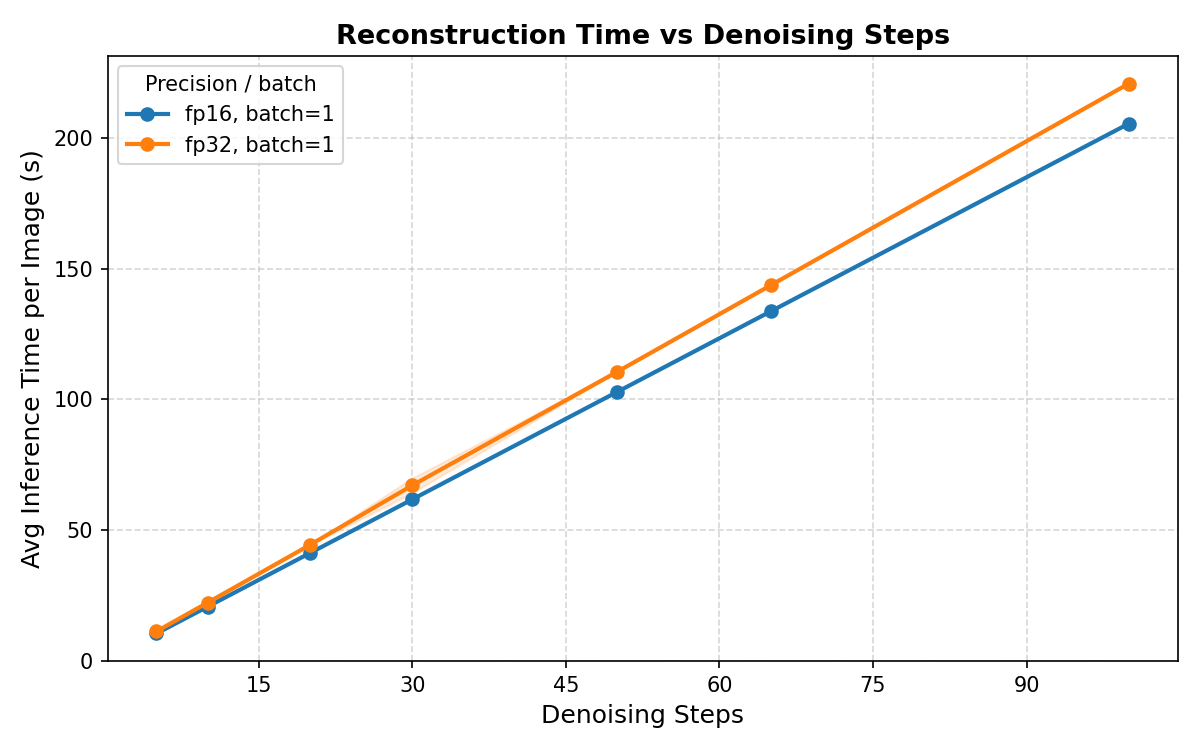
\includegraphics[width=\linewidth]{reconstruction_time_vs_steps.png}
\caption{Reconstruction time increases nearly linearly with denoising steps in the full-image DeltaAI GH200 profile.}
\label{fig:time-steps}
\end{figure}

\subsection{Tiling Reduces Memory and Runtime}

The first tiling pilot showed that a $512 \times 512$ tile reduced time from 143.55 to 86.01 seconds per image and peak GPU memory from 52.0 GB to 3.0 GB. The later selected validation compared no tiling, $256 \times 256$ tiling, and $512 \times 512$ tiling on 50 full-resolution images. Table~\ref{tab:tiling} shows the selected result.

\begin{table*}[t]
\caption{Selected DeltaAI GH200 tiling validation on 50 full-resolution images, 65 denoising steps, fp32.}
\label{tab:tiling}
\centering
\begin{tabular}{l r r r r r r r}
\hline
Setup & Sec./image & GB & Ratio & PSNR & SSIM & MAE & Error p99\\
\hline
No tiling & 144.35 & 52.01 & 70.11$\times$ & 28.96 & 0.8616 & 0.027016 & 0.117676\\
$256 \times 256$ tile & 79.84 & 1.66 & 68.24$\times$ & 28.78 & 0.8552 & 0.027463 & 0.120211\\
$512 \times 512$ tile & 87.71 & 3.02 & 66.31$\times$ & 28.86 & 0.8583 & 0.027246 & 0.118897\\
\hline
\end{tabular}
\end{table*}

The $256 \times 256$ setting is the best speed and memory candidate in the selected run. It reduces wall time by 44.7\% and peak GPU memory by about 31.3$\times$ relative to no tiling. Compared with $512 \times 512$ tiling, it is about 9.0\% faster and uses about 45.0\% less GPU memory. The quality trade-off is small in scalar metrics: compared with $512 \times 512$, PSNR drops by 0.086 dB, SSIM drops by 0.0031, and the 99th percentile absolute error increases by 0.001314.

\begin{figure*}[t]
\centering
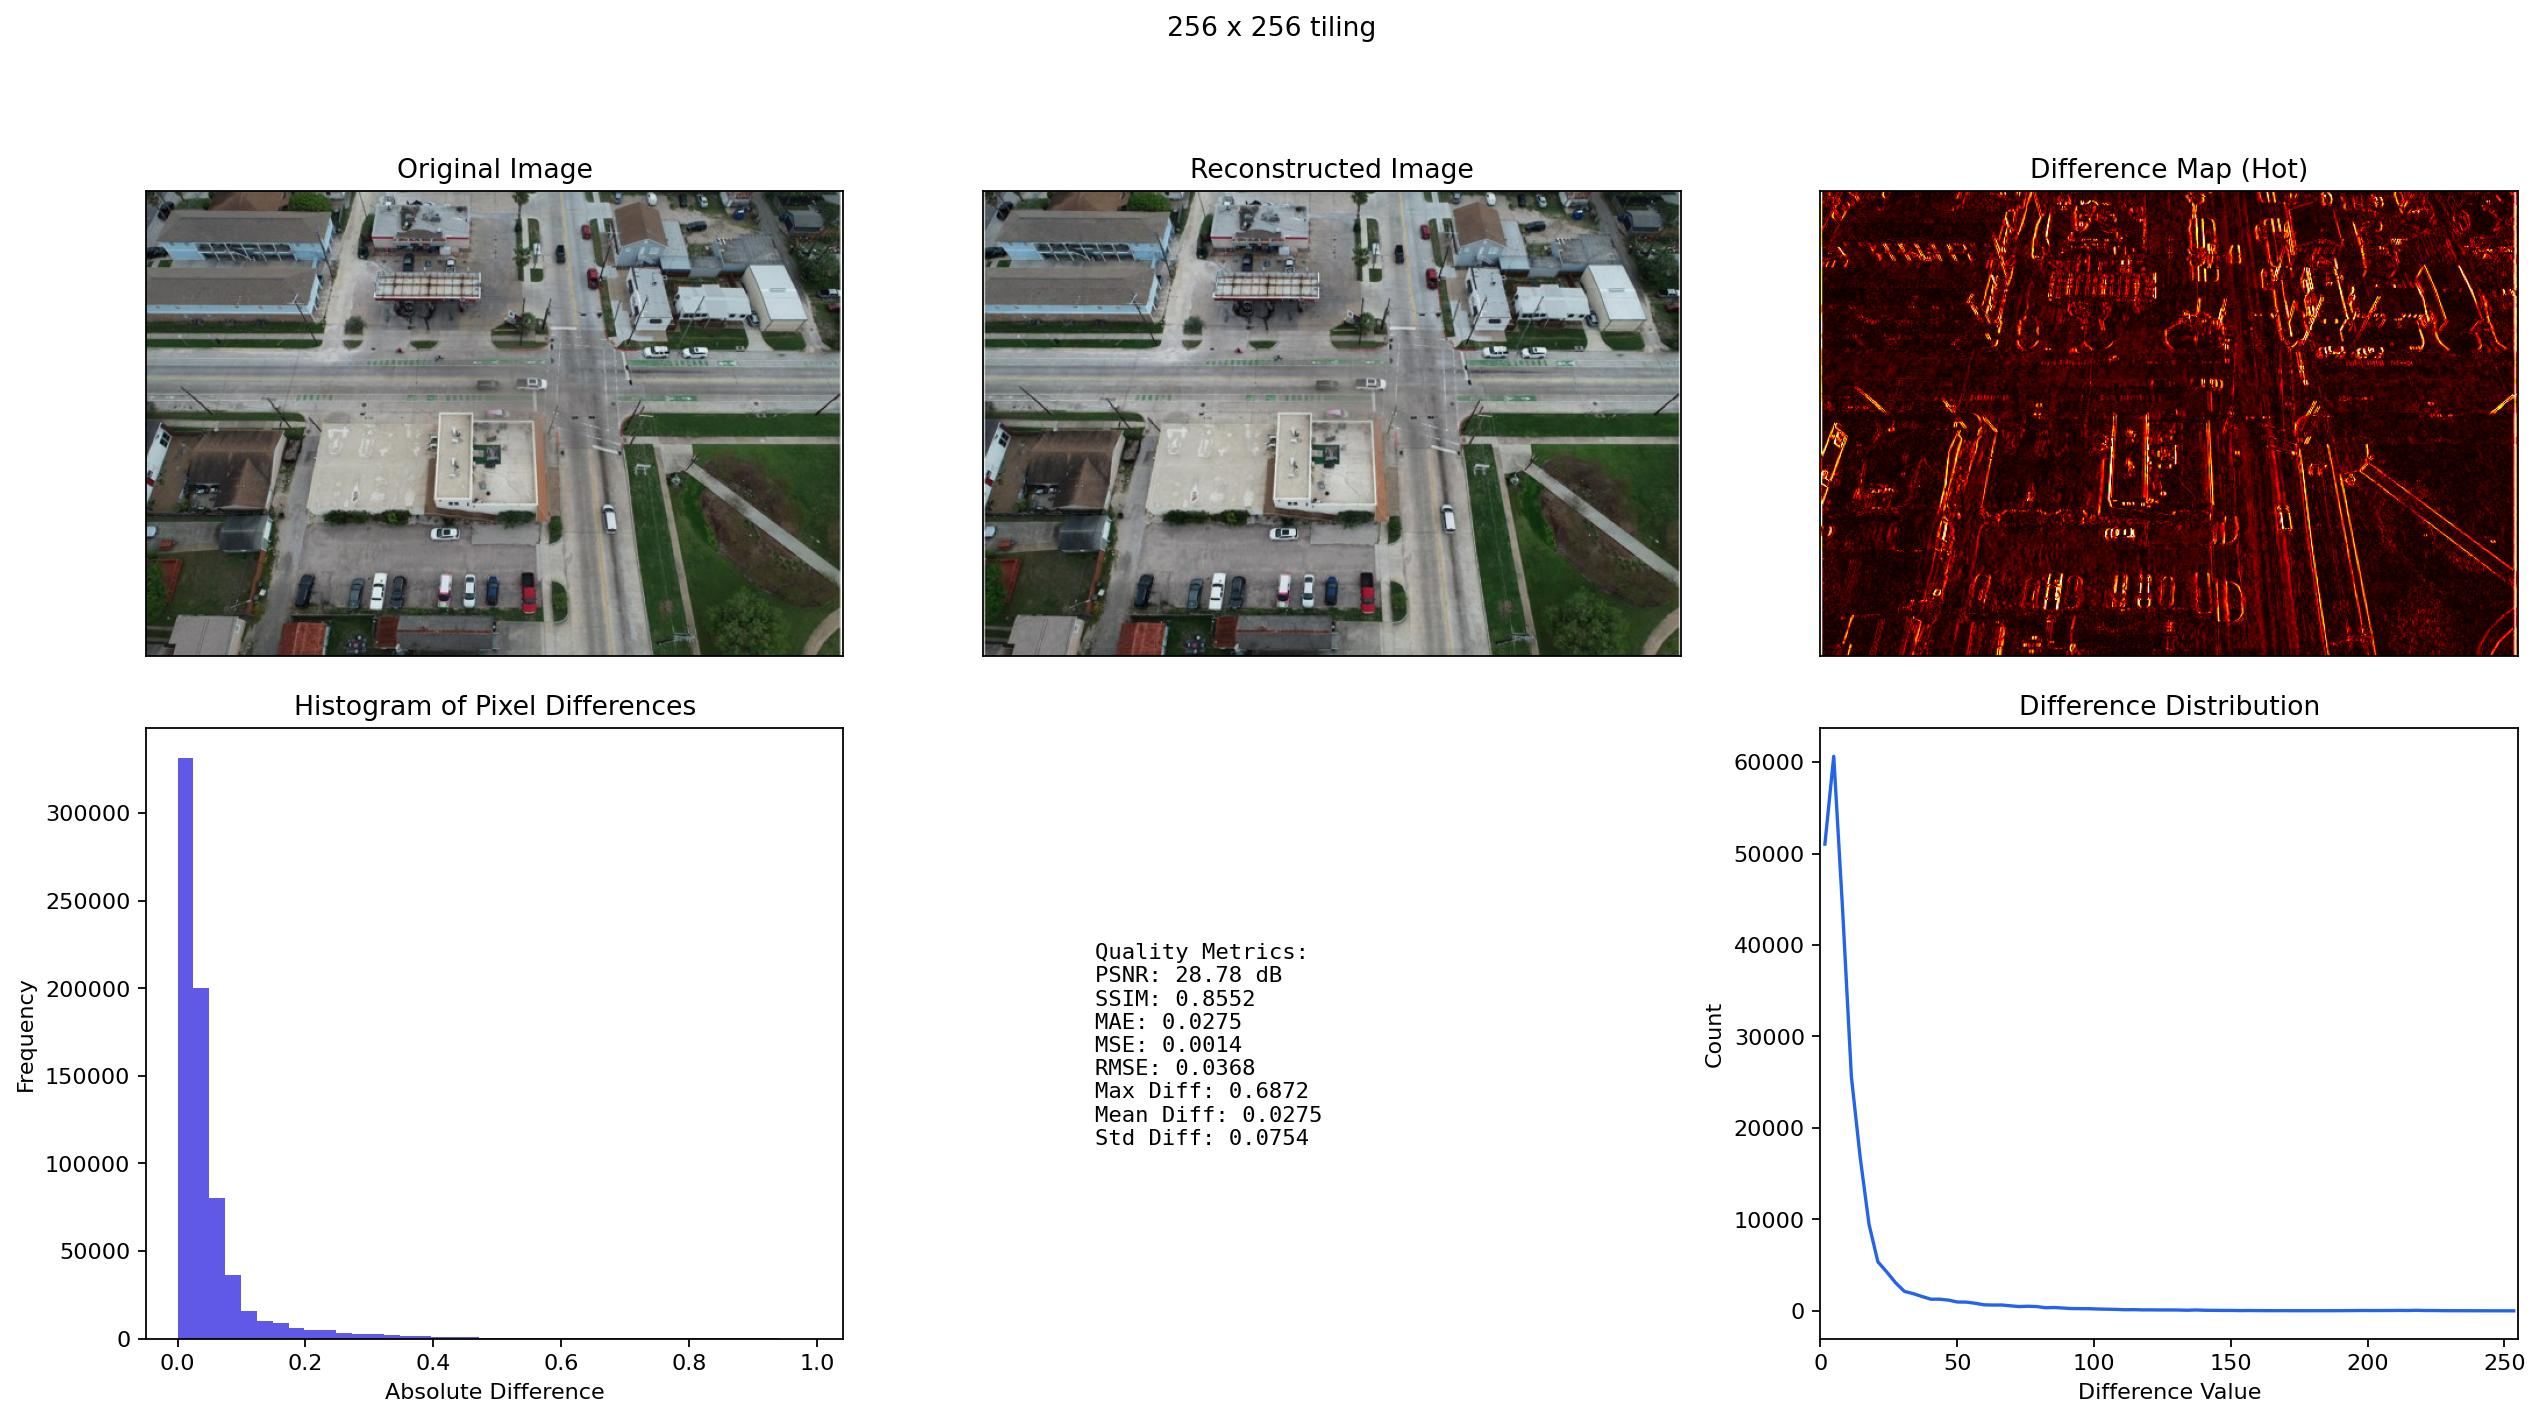
\includegraphics[width=0.86\textwidth]{tile256_poster_panel.jpg}
\caption{Poster-ready visual QA panel for the selected $256 \times 256$ tiling case. The panel combines original preview, reconstruction, hot difference map, pixel-difference histogram, metric text, and difference distribution for a representative image.}
\label{fig:tile-panel}
\end{figure*}

\subsection{Resolution Reduction Is Fast but Quality-Limited}

Resolution reduction provides the largest raw speedup, but it changes the image content available to downstream tasks. In the compression-side validation, reducing the longest edge to 4K lowered time from 144.32 to 28.89 seconds per image and memory from 52.0 to 29.0 GB. Reducing to 2K lowered time to 7.36 seconds and memory to 7.47 GB, but SSIM dropped to 0.689. The 1K setting was faster again, but the quality loss was too large for detailed disaster-imagery inspection.

\begin{table}[t]
\caption{Resolution sweep on DeltaAI GH200, 20 images, baseline checkpoint.}
\label{tab:resolution}
\centering
\begin{tabular}{l r r r r r}
\hline
Resolution & Sec. & GB & Ratio & PSNR & SSIM\\
\hline
Native & 144.32 & 52.00 & 71.20$\times$ & 29.45 & 0.873\\
4K & 28.89 & 28.98 & 72.92$\times$ & 28.26 & 0.847\\
2K & 7.36 & 7.47 & 81.31$\times$ & 24.05 & 0.689\\
1K & 1.94 & 2.01 & 77.83$\times$ & 21.95 & 0.610\\
\hline
\end{tabular}
\end{table}

\subsection{Batching Does Not Improve the 2K Controlled Run}

The controlled 2K batch-size sweep shows that larger batches do not improve throughput in the current implementation. Batch size 1 runs at 7.35 seconds per image and uses 7.47 GB of GPU memory. Batch size 2 slows to 11.60 seconds per image and uses 14.64 GB. Batch size 4 improves over batch size 2 but remains slower than batch size 1 while using 28.96 GB. These results support batch size 1 as the default for the current workflow.

\subsection{Checkpoint Selection Controls the Storage-Quality Trade-Off}

Because the x-parameterized path does not expose a direct runtime quality parameter, the practical compression level comes from checkpoint selection. Table~\ref{tab:checkpoints} summarizes representative checkpoints. Runtime stays near 144 seconds per image for all listed checkpoints, while compression ratio and quality change substantially. The strongest listed compression setting, \texttt{checkpoint\_b00128}, reaches 165.73$\times$ compression with lower SSIM. The \texttt{checkpoint\_b00512} setting has the highest SSIM in this table and a lower compression ratio. The \texttt{checkpoint\_b00064} setting provides a middle operating point with 93.11$\times$ compression and SSIM 0.880.

\begin{table}[t]
\caption{Checkpoint-controlled compression settings on native full-resolution images, 20-image validation.}
\label{tab:checkpoints}
\centering
\begin{tabular}{l r r r r}
\hline
Checkpoint & Sec. & Ratio & PSNR & SSIM\\
\hline
\texttt{b00512} & 143.73 & 32.67$\times$ & 34.84 & 0.942\\
\texttt{b00064} & 143.66 & 93.11$\times$ & 33.73 & 0.880\\
\texttt{b00128} & 143.70 & 165.73$\times$ & 31.52 & 0.828\\
\texttt{b02048} & 143.70 & 71.20$\times$ & 29.45 & 0.873\\
\hline
\end{tabular}
\end{table}

\subsection{Storage Placement Has Little Effect in the Current Run}

The storage comparison showed almost no difference between shared filesystem access and node-local staged input for the native baseline. Shared storage took 143.86 seconds per image, while local staging took 143.89 seconds per image. This result suggests that the current workflow is compute-bound under the tested configuration. It does not rule out I/O effects for larger concurrent runs, but it makes local staging a lower-priority optimization than tiling, denoising-step control, and checkpoint selection.

\section{Discussion}

The main result is that the full-resolution CDC workflow is feasible on DeltaAI GH200 but inefficient if it processes each image as one native tensor. The baseline uses about 52 GB of GPU memory per image and takes about 144 seconds per image at 65 denoising steps. That operating point is acceptable for a small validation set, but it is too expensive for repeated large disaster-imagery archives.

Tiling changes the cost profile. The $256 \times 256$ setting keeps the same native image dimensions at the workflow boundary, but it moves most of the computation to small tile tensors. That choice cuts peak memory from 52.01 GB to 1.66 GB and lowers time from 144.35 to 79.84 seconds per image. The quality metrics decline slightly, but the change is modest compared with the memory reduction. The remaining risk is visual: small scalar changes do not guarantee that tile seams are invisible. For that reason, the visual QA panel is not decorative. It is part of the evidence needed to accept a tiled operating point.

Resolution reduction provides a different kind of saving. It is much faster than tiling, but it also removes spatial detail before compression. For workflows that only need coarse scene context, 2K or 1K inputs may be adequate. For damage assessment, object localization, and visual evidence, however, the quality drop in the 2K and 1K rows is likely too large unless downstream task accuracy confirms otherwise.

Checkpoint selection should be treated as a first-class experimental control. The current x-parameterized workflow does not support a simple runtime compression-level parameter. Reporting only a checkpoint name would make the result hard to interpret, so this draft reports checkpoint, BPP-derived compression ratio, PSNR, and SSIM together. The checkpoint sweep also shows that runtime is not the main differentiator across compression settings; the main change is the storage-quality trade-off.

The study has several limitations. The sample sizes are small, and the current visual QA uses selected representative examples. The experiments report image-quality metrics rather than downstream disaster-analysis accuracy. The fp16 path is promising for memory and speed but cannot yet be used for BPP-based reporting because the current output records invalid BPP values. Finally, the Delta H200 comparison is only a quick check and should not be treated as a full cross-system benchmark.

\section{Conclusion}

This paper turns a CDC image-compression model into a measurable HPC workflow for 4K-5K drone imagery. The experiments show that native full-image CDC processing on DeltaAI GH200 is feasible but expensive, while tiled processing is a practical path toward lower memory and faster turnaround. The selected $256 \times 256$ tiling configuration reduces runtime by 44.7\% and peak GPU memory by about 31.3$\times$ relative to no tiling on 50 full-resolution images, with small scalar quality losses relative to $512 \times 512$ tiling. For the next draft, the highest-value additions are a full related-work section, larger validation runs, downstream task checks, and a visual artifact audit across more images.

\section*{Acknowledgment}

The authors thank the NCSA DeltaAI support ecosystem and project collaborators for discussions that shaped the experiment design.

\bibliographystyle{IEEEtran}
\bibliography{references}

\end{document}
